\section{Economic Analysis}
\phantomsection

\subsection{Project description}

Nowdays social media become an important marketing tool. Beside a big network where everyone can share information and express their thougts, social media channels represent a good place for advertising different types of products and services. These special types of posts are called blogs. In this context people start to use social media as a source of inspiration regarding questions like: how to dress? what to cook? how to loose weight? what products to use for skin? Together with people interest about blogs, increased and interest of companies who provides products and services.

MyApp represents a tool which will help companies to find influential bloggers according to their preferences.

\subsection{Project time schedule}

For a better development of the project a well defined time schedule is needed. The most suitable approach for MyApp application is agile project management, because it focuses on continuous improvement. It consists of several iterations, each interation has 5 steps: planning, research, development, testing and deployment.

\subsubsection{Objective determination}

During the first step of agile project management -- planning -- a set of objectives are established in order to determine what the project is supposed to accomplish when ended. Without a well defined objectives it is impossible to evaluate the results and to plan the activities for achieving them. This is the reason why objectives should be SMART. 

The main goal of the project is to give stakeholders a list of influential bloggers, according to their requirements, with estimated impact regarding product visibility.

The key objectives that should be meet in order to achieve the goal are:

\begin{itemize}

\item[--] \textit{To organize information from the database into well defined categories.} This objective is crucial, because social media content represents an unstructured data and it is hard to analyse it in the raw form. Organizing information by categories will lead to a better processing.

\item[--] \textit{To create dependeces between categories.} Not all the words can be set as an independent category. That's why a category tree, which includes subcategories, should be created for each category.

\item[--] \textit{To develop a search mechanism according to specified requirements.} The results obtained after search should be as specific as possible, meeting all requirements as stated by user.

\item[--] \textit{To filter the resulting list and to keep only the influential bloggers.} Since the big amount of data, the resulting list after search should be huge, containing also bloggers not so influnetial. A filter according to numbers of views, reviews and numbers of subscribes have to be done.

\item[--] \textit{To estimate the impact of choosing that specific bloger as a promoter.} Beside a list of names, the application should offer an impact estimation regarding product visibility.

\end{itemize}

\subsubsection{Time schedule establishment}

Project scheduling consists of three main parts: what activity needs to be performed, the number of days in which it should be performed and which people are responsible for it. The time schedule is divided according to specified agile project management steps. Thus, for planning and researching phases there is not a strict ammount of time and a well determined splitting, because the requirements may change and the process of analysing should be repeated. The same thing can not be assumed for development step, where the process is splited up in smaller tasks with a defined period of days. To be able to compute the total duration of the project the formula \eqref{eq:duration} is used.

\begin{equation} \label{eq:duration}
 D_T = D_F - D_S + T_R,
\end{equation}

\noindent
where $D_T$ is the duration, $D_F$ -- the finish date, $D_S$ -- the start date and $T_R$ -- reserve time. The first iteration of the project schedule is presented in Table \ref{table:schedule}. To define the people working on the project the following notations are used: PM -- project manager, SA -- system architect, SM -- sales manager, D -- developer.

\begin{table}[!ht]
\begin{center}
\caption{Time schedule}
\renewcommand{\arraystretch}{2}
\begin{tabular}{| c | >{\centering\arraybackslash}p{7.5cm}  | >{\centering\arraybackslash}p{5cm} | c |}
\hline
\textbf{Nr} & \textbf{Activity Name} & \textbf{Duration (days)} & \textbf{People involved}  \\
\hline
1 & Project specification and business processes & 6 & PM, SA, SM, D  \\
\hline
2 & Analysis of market & 10 & PM, SA  \\
\hline
3 & Analysis of the domain & 14 & SA, D  \\
\hline
4 & Requirements analysis and catalogue & 5 & PM, SA, D  \\
\hline
5 & System design (UML) & 12 & PM, SA, D  \\
\hline
6 & Database design & 7 & PM, SA, D \\
\hline
7 & Specification and analysis of architectue and technologies & 20 & PM, SA, D \\
\hline
8 & End-user application development & 30 & PM, SA, D, SM  \\
\hline
9 & Validation of results & 10 & PM, SA, D, SM  \\
\hline
10 & Documentation & 7 & D  \\
\hline
11 & Deployment and testing & 10 & PM, SA, D  \\
\hline
12 & Active marketing & 7 & SM  \\
\hline
13 & Total time to finish the system & 138 &  \\
\hline
\end{tabular}
\label{table:schedule}
\vspace{-2.5em}
\end{center}
\end{table}

Table \ref{table:schedule} describes in the main activities during first iteration of the project together with number of days allocated per activity. By summing these days we get a total amount of time of 138 days nedded to complete the project.

\subsection{Economic motivation}

In this section the project is evaluated from an economic point of view, which implies a measure of its net benefits in monetary terms (MDL (Moldavian lei) currency) by using real or estimated market prices. During analysis all expenditures incurred under the project like: tangible and intangible assets, direct and salary expenses,  and revenues resulting from it are taken into acount.

\subsubsection{Tangible and intangible asset expenses}

In Table \ref{table:tangible_assets} are listed tangible assets and their expenses. The term tangible asset means an asset that has a physical form, such as machinery.

\begin{table}[!hb]
\begin{center}
\caption{Tangible asset expenses}
\renewcommand{\arraystretch}{2}
\begin{tabular}{| >{\centering\arraybackslash}p{1.7cm}  | >{\centering\arraybackslash}p{5cm} | >{\centering\arraybackslash}p{2.7cm} | >{\centering\arraybackslash}p{2cm} | c | >{\centering\arraybackslash}p{5em}|}
\hline
\textbf{Material} & \textbf{Specification} & \textbf{Measurement unit} & \textbf{Price per unit (MDL)} & \textbf{Quantity} & \textbf{Sum (MDL)}\\
\hline
Lenovo ideapad & i5 & Unit & 12000 & 1 &  \multicolumn{1}{r|}{12000}\\
\hline
\multicolumn{5}{|r|}{Total} & \multicolumn{1}{r|}{12000}\\
\hline
\end{tabular}
\label{table:tangible_assets}
\end{center}
\vspace{-1.3em}
\end{table}

The budget for the required intangible assets, i.e., nonphysical assets, such as patents, trademarks, copyrights brand recognition, is shown in Table \ref{table:intangible_assets}.

\begin{table}[!hb]
\begin{center}
\caption{Intangible asset expenses}
\renewcommand{\arraystretch}{2}
\begin{tabular}{| c | >{\centering\arraybackslash}p{5cm} | >{\centering\arraybackslash}p{2.7cm} | >{\centering\arraybackslash}p{2cm} | c | >{\centering\arraybackslash}p{5em}|}
\hline
\textbf{Material} & \textbf{Specification} & \textbf{Measurement unit} & \textbf{Price per unit (MDL)} & \textbf{Quantity} & \textbf{Sum (MDL)} \\
\hline
License & Enterprise Architect Desktop Edition License & Unit & 1900 & 3 & \multicolumn{1}{r|}{5700} \\
\hline
\multicolumn{5}{|r|}{Total} & \multicolumn{1}{r|}{5700}\\
\hline
\end{tabular}
\label{table:intangible_assets}
\vspace{-1em}
\end{center}
\end{table}

Direct expenses are presented in Table \ref{table:direct_expenses}. It includes purchase of raw materials used during planing, analysing and meetings. These expenses are indispensable in every project at any stage.

So the total amount of direct expenses in MDL is:

\begin{equation}
 T_e = 12000 + 5700 = 17700
\end{equation}

\begin{table}[!hb]
\begin{center}
\caption{Direct expenses}
\renewcommand{\arraystretch}{2}
\begin{tabular}{| >{\centering\arraybackslash}p{7.5em} | >{\centering\arraybackslash}p{8em} | >{\centering\arraybackslash}p{7em} | >{\centering\arraybackslash}p{5em} | >{\centering\arraybackslash}p{5em} | r |}
\hline
\textbf{Material} & \textbf{Specification} & \textbf{Measurement unit} & \textbf{Price per unit (MDL)} & \textbf{Quantity} & \multicolumn{1}{>{\centering\arraybackslash}p{5em}|}{\textbf{Sum (MDL)}}\\
\hline
Whiteboard & Universal Dry Erase Board & Unit & 500 & 1 & 500 \\
\hline
Paper & A4 & 250 sheets & 60 & 1 & 60 \\
\hline
Marker & Whiteboard marker & Unit & 15 & 5 & 75 \\
\hline
Eraser & Whiteboard eraser & Unit & 60 & 2 & 120 \\
\hline
Pen & Blue pen & Unit & 5 & 10 & 50 \\
\hline
Flipchart paper & A1 & 80sheets & 75 & 2 & 150 \\
\hline
Tape & Paper tape & Unit & 6 & 2 & 12 \\
\hline
Marker & Permanent marker & Unit & 10 & 5 & 50 \\
\hline
\multicolumn{5}{|r|}{Total} & 1017 \\
\hline
\end{tabular}
\label{table:direct_expenses}
\vspace{-1.5em}
\end{center}
\end{table}

\subsubsection{Salary expenses}

This section includes the budget which is allocated for employee remuneration. As specified above on the project will work 4 people and according to their position a different amount of money will be paid per day, as shown in Table {table:salaries}.

\begin{table}[!ht]
\begin{center}
\caption{Salary expenses}
\renewcommand{\arraystretch}{2}
\begin{tabular}{| >{\centering\arraybackslash}p{8em} | >{\centering\arraybackslash}p{8em} | >{\centering\arraybackslash}p{8em} | r |}
\hline
\textbf{Employee} & \textbf{Work fund (days)} & \textbf{Salary per day (MDL)} & \multicolumn{1}{>{\centering\arraybackslash}p{5em}|}{\textbf{Salary fund (MDL)}}\\
\hline
Project Manager & 120 & 350 & 42000 \\
\hline 
System Architect & 90 & 400 & 36000\\
\hline
Sales Manager & 60 & 250 & 15000\\
\hline
Developer & 120 & 330 & 39600\\
\hline
\multicolumn{3}{|r|}{Total} & 132600\\
\hline
\end{tabular}
\label{table:salaries}
\vspace{-2.5em}
\end{center}
\end{table}

Since, the project involves employees it is necessary to compute how much should be paid to medical insurance, social services fund and the total work expenses.

The medical insurance fund is calculated as:

\begin{equation}
\begin{split}
 MI &= F_{re} \cdot T_{mi}\\ 
    &= 132600 \cdot 0.035\\ 
    &= 4641,
 \end{split}
\end{equation}

\noindent
where $T_{mi}$ is the mandatory medical insurance tax and this year it is $3.5\%$. 

The social fund for this year is 23\%, thus the salary expenses are computed as follows:

\begin{equation}
\begin{split}
 FS &= F_{re} \cdot T_{fs} \\
    &= 132600 \cdot 0.23 \\
    &= 30498,
\end{split}
\end{equation}

\noindent
where $FS$ is the salary expense, $F_{re}$ is the salary expense fund and $T_{fs}$ is the social service tax.

Having all the calculations done for social service tax and medical insurance tax, it is possible to found out total work expense using the relation \eqref{eq:total_work_expense}

\begin{equation}\label{eq:total_work_expense}
\begin{split}
 WEF &= F_{re} + FS + MI\\
     &= 132600 + 30498 + 4641\\
     &= 167739,
\end{split}
\end{equation}

\noindent
where $WEF$ is the work expense fund, FS -- the social fund and MI -- the medical insurance fund.

\subsection{Individual person salary}

Besides total salary expenses, it is necessary to compute the annual individual person salary. For this we'll take the employee which has the bigest salary -- system architect. Considering that the system architect has a salary of 400 MDL per day and the number of working days in the year is equal to 250, so the gross salary that the system architect get is calculated as: 

\begin{equation} 
 GS = 400 \cdot 250 = 100000,
\end{equation}

\noindent
where \textit{GS} is the gross salary in MDL.

The gross salary is computed before any deductions are taken for state and federal taxes, social and health insurance. 

Social fund tax represents 6 \% of the total amount, so the taxt that should be paid in MDL represents

\begin{equation}
 SF = 100000 \cdot 0.06 = 6000,
\end{equation}

Medical insurance tax represents 4.5 \% and the required amount that should be paid is

\begin{equation}
 MIF = 100000 \cdot 0.045 = 4500,
\end{equation}

To be able to procced with income tax computations, first it is needed to calculate the amount of taxed salary using the relation \eqref{eq:taxed_salary}

\begin{equation}\label{eq:taxed_salary}
\begin{split}
 TS  &= GS - SF - MIF - PE\\
     &= 100000 - 6000 - 4500 - 10128\\
     &= 79372,
\end{split}
\end{equation}

\noindent
where \textit{TS} is the taxed salary, \textit{GS} -- gross salary, \textit{SF} -- social fund and \textit{PE} -- personal exemption, which is approved every year. This year the amount is of 10128. 

One more thing that should be computed regarding taxes is the total income tax. It represents 7 \% for income under 29640 MDL and 18 \% for income over 29640 MDL. 

\begin{equation}
\begin{split}
 IT  &= TS - ST\\
     &= 29640 \cdot 0.07 + (79372 - 29640) \cdot 0.18\\
     &= 2074.8 + 8951.76 = 11026.56,
\end{split}
\end{equation}

\noindent
where \textit{IT} is the income tax, \textit{TS} represents taxed salary and \textit{ST} -- the salary tax. 

Now all the indices are computed and it is possible to find out the amount of net income. 

\begin{equation}
\begin{split}
 NS  &= GS - IT - SF - MIF\\
     &= 100000 - 11026.56 - 6000 - 4500\\
     &= 78473.44,
\end{split}
\end{equation}

\noindent
where \textit{NS} is the net salary, \textit{GS} -- gross salary, \textit{IT} -- income tax, \textit{SF} -- social fund and \textit{MIF} the medical insurance fund. 

\subsubsection{Indirect expenses}

Every complex project involves indirect expenses, that are inevitable, such as electricity, water, Internet traffic, etc. All the expenses are represented in Table \ref{table:indirect_expenses}.

\begin{table}[!ht]
\begin{center}
\caption{Indirect expenses}
\renewcommand{\arraystretch}{2}
\begin{tabular}{| >{\centering\arraybackslash}p{5em} | >{\centering\arraybackslash}p{7em} | >{\centering\arraybackslash}p{7em} | >{\centering\arraybackslash}p{5em} | >{\centering\arraybackslash}p{5em} | r |}
\hline
\textbf{Material} & \textbf{Specification} & \textbf{Measurement unit} & \textbf{Price per unit (MDL)} & \textbf{Quantity} & \multicolumn{1}{>{\centering\arraybackslash}p{4em}|}{\textbf{Sum (MDL)}}\\
\hline
Internet & StarNet & Pack & 200.00 & 3 & 600 \\
\hline
Transport & Public bus & Trip & 3.00 & 150 & 450\\
\hline
Phone & Moldtelecom & Pack & 30.00 & 3 & 90\\
\hline
Electricity & Union Fenosa & KWh & 2.16 & 500 & 1080\\
\hline
\multicolumn{5}{|r|}{Total} & 2220 \\
\hline
\end{tabular}
\label{table:indirect_expenses}
\vspace{-2.5em}
\end{center}
\end{table}

\subsubsection{Wear and depreciation}

This part is crucial in economic analysis process, because the monetary value of an asset decreases over time due to use, wear and tear. The descrease is measured as depreciation. Depreciation may be caused by unfavorable market conditions, machinery equipment or currency, that are likely to decrease over a specific period of time. 

The depreciation expense is calculated using the straight line depreciation method by spreading the cost evenly over the life of the fixed asset. In order to do this, the asset's lifespan and salvage value need to be known. The expected lifespan of the purchased asset depends on the type. For example, the notebook and single-board computer are usable for a period of 3 years. Salvage value of the item represents how much it will be worth once it's outlived its usefulness. 

First step in computing the depreciation is to calculate the total asstes value, using relation \eqref{eq:tav}. For this are summed up the tangible and intangible asstes and then the salvage costs has to be substracted. 

\begin{equation}\label{eq:tav}
 \begin{split}
  TAV &= \sum_{} (AC - SV) \\
        &= (12000 - 1000) + (5700 - 1000) \\
        &= 13700,
 \end{split}
\end{equation}

\noindent
where \textit{TAV} is the total assets value, \textit{AC} -- assets costs and \textit{SV} -- salvage value.

Second step is to get the yearly wear. To do this is need to divide total asset value by the asset's lifespan, that is 3 years.

\begin{equation}
 \begin{split}
  W_{y} &= TAV/T{use} \\
        &= 13700/3 \\
        &= 4567,
 \end{split}
\end{equation}

\noindent
where $W_{y}$ represents the wear per year, \textit{TAV} -- total assets value and $T{use}$ the asste's lifespan. 

The initial value of assets in MDL was

\begin{equation}
 \begin{split}
  W &= W_{y}/D_{y} \cdot T_{p} \\
    &= 4567/365 \cdot 138 \\
    &= 1726.7,
 \end{split}
\end{equation}

\subsubsection{Product cost}

Product cost refers to the costs used to create a product. These costs inlude all the expenses analysed before as shown in Table \ref{table:product_cost}.

\begin{table}[!ht]
\begin{center}
\caption{Total Product Cost}
\renewcommand{\arraystretch}{2}
\begin{tabular}{| >{\centering\arraybackslash}p{10em} | r | r |}
\hline
\textbf{Expense type} & \multicolumn{1}{>{\centering\arraybackslash}p{6em}|}{\textbf{Sum (MDL)}} & \multicolumn{1}{>{\centering\arraybackslash}p{6em}|}{\textbf{Percentage (\%)}}\\
\hline
Direct expenses & 1017 & 0.75 \\
\hline
Indirect expenses & 2220 & 1.61 \\
\hline
Salary expenses & 132600 & 96.3 \\
\hline
Asset wear expenses & 1726.7 & 1.25 \\
\hline
\textbf{Total product cost} & \textbf{137563.7} & \textbf{100}\\
\hline
\end{tabular}
\label{table:product_cost}
\vspace{-2.5em}
\end{center}
\end{table}

\subsubsection{Economic indicators and results}

Now, when all the expenses are calculated it is necessary to understand and implement and effective selling strategie. First step in this sense is to understand target customers. The key customers of MyApp are brand companies. To make them know about the product a good advertising is crucial. That implies additional costs and finding an investor will be the best solution in this case.  

At the moment the tool does not have a fixed price, thus for determining the aproximated price the 25 \% on top of the production cost principle is used. 

\begin{equation}
 \begin{split}
  GP &= C_{total} / N_{cs} + P_{p}\\
              &= 137563.7/100 + 25 \% \\
              &= 1719.54,
 \end{split}
\end{equation}

\noindent
where \textit{GP} is the gross price, $C_{total}$ the total product cost, $N_{cs}$ the number of copies sold and $P_{p}$ chosen profit precentage. 

The price of the end product has sales tax (VAT) included, so it to the computed gross price is added the sales tax, which represents 20 \%. Using relation \ref{eq:sale_price} the sale price including VAT is computed

\begin{equation}\label{eq:sale_price}
 \begin{split}
  P_{sale} &= GP / TX{sales}\\
           &= 1719.54 + 20 \% \\
           &= 2063.5,
 \end{split}
\end{equation}

\noindent
where $GP$ is the gross price and $TX_{sales}$ the sales tax. 

Besides sale price, other economic indicators, like: net income, gross and net profit, cost profitability and sales profitability are important and should be computed. 

Net income is a distinct accounting concept from profit. Net income is calculated by multiplying gross price and the numer of expected copies to be sold. The expected amount of copies to be sold is 100.

\begin{equation}
 \begin{split}
  I_{net} &= GP \cdot N_{cs}\\
          &= 1719.54  \cdot 100 \\
          &= 171954,
 \end{split}
\end{equation}

\noindent
where $GP$ -- gross price and $N_{cs}$ -- number of copies sold.

Gross profit is a company's total revenue (equivalent to total sales) minus the cost of goods sold. Together with it is also calculated the net profit. 

\begin{equation}
 \begin{split}
  GPr &= I_{net} - C_{production}\\
      &= 171954 - 137563.7\\
      &= 34390.3 \\
  NPr &= GPr - 12\% \\
      &= 34390.3 - 12\% \\
      &= 30263.46,
 \end{split}
\end{equation}

\noindent
where $I_{net}$ is the net income and $C_{production}$ -- cost of production.

Profitability indicators are a class of financial metrics that are used to assess a business's ability to generate earnings as compared to its expenses and other relevant costs incurred during a specific period of time. There are two types of indicators that are calculated for the project $C_{profit}$ -- cost profitability, $S_{profit}$ -- sales profitability.

\begin{equation}
 \begin{split}
  C_{profit} &= GPr / C_{production} \cdot 100\%\\
             &= 34390.3 / 137563.7 \cdot 100\% \\
             &= 24.99 \%\\
  S_{profit} &= GPr / I_{net} \cdot 100\% \\
             &= 34390.3 / 171954 \cdot 100\% \\
             &= 19.99 \%.
 \end{split}
\end{equation}

\subsection{Marketing Plan}

The term of marketing means the management process through which goods and services move from concept to the customer. American Marketing Association defined it as ``the activity, set of institutions, and processes for creating, communicating, delivering, and exchanging offerings that have value for customers, clients, partners, and society at large." \cite{marketing} 

The traditional way of viewing the components of marketing is using the four Ps:

\begin{enumerate}

\item \textbf{Product} -- creating offerings.
\item \textbf{Promotion} -- developing and implementing strategy.
\item \textbf{Place} -- selecting the right distribution channel to reach the customers.
\item \textbf{Price} -- determining the monetary amount for the product.

\end{enumerate}

These four components are part of the marketing plan.

For the MyApp project marketing plan is crutial, because the product should be promoted among potential customers. The marketing plan is be based on where the project needs to be at some point in the future.

It includes several key componnets: 
\begin{enumerate}

\item[--] \textbf{Market Research:} identify consumer buying habits in the industry, market size, market growth or decline, and any current trends.

\item[--] \textbf{Target Market:} find target markets for the product and describe them.

\item[--] \textbf{Positioning:} define the perception of the product in the marketplace.

\item[--] \textbf{Competitive analysis:} research competitors and describe why your product is better.

\item[--] \textbf{Market strategy:} describe marketing and promotion strategies that will be used, like: direct marketin (sales letters, flyers), web site, advertising (print media), direct/personal selling.

\item[--] \textbf{Budget:} a month-by-moth schedule of what is plan to be spend on marketing.

\item[--] \textbf{Matrics:} establish quantifiable marketing goals. This means goals that you can turn into numbers.

\end{enumerate}

Another aspect that should be taken into consideration is the product life cycle. A new product progresses theough a sequence of stages from introducion to growth, maturity and decline, as shown in Figure \ref{product-stage}. It is important to know the caracterics of each stage in order to take corresponding actions regarding the situation.

\begin{figure}[!ht]
\centering
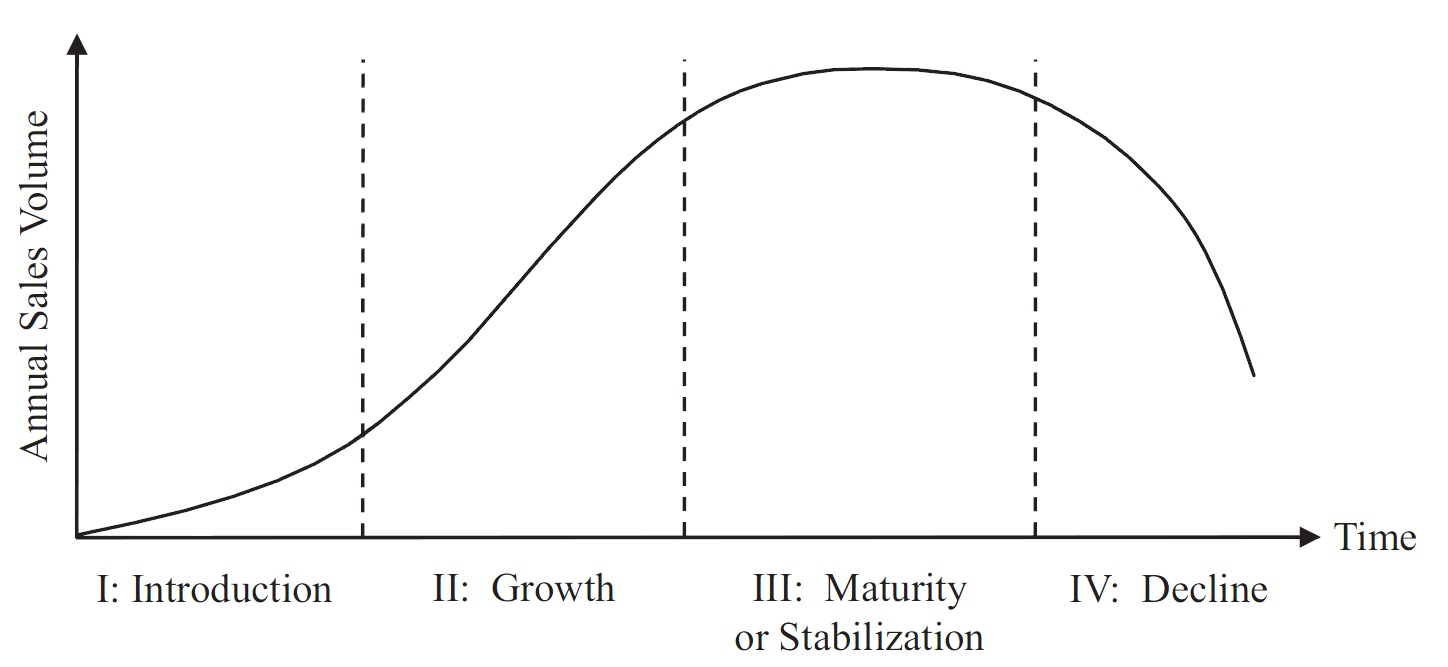
\includegraphics[width=10cm]{product-life-cycle}
\caption{Product Life Cycle Diagram\cite{prodcutFigure}}\label{product-stage}
\end{figure}


\begin{itemize}

\item[--] \textbf{Introduction Stage.} The most expensive stage. The size of the market for the product is small, thus sales are low. It is need to build product awareness and to develop a market for the product.

\item[--] \textbf{Growth Stage.} The stage is characterized by a strong growth in sales and profits. There is neccessary to build brand preference and increase market share.

\item[--] \textbf{Maturiy Stage.} Strong growth in sales. The objective at this point is to defend and maintain the market share while maximizing profit. 

\item[--] \textbf{Decline Stage.} The market for the product start to shrink and sales to decline. At this stage the company should decide what to do further: 

\begin{itemize}

\item Maintain the product (adding new features and finding new uses).

\item Harvest the product (reduce costs and niche segment).

\item Discontinue the product (liquidate or sell it to another firm).\cite{stages}

\end{itemize}
\end{itemize}

\subsection{Economic conclusions}

In this chapter MyApp project was analyzed in economic terms. The analysis was done to assess the opportunity of the project by considering the benefits compared to the costs. Besides financial indicators, other additional aspects as market influences, social and envrironmental costs were considered. 

The product at introduction stage is very hard to promote. It is necessary to set up a well defined set of objectives and to develope a detailed marketing plan. The company should investigate all threats and have a plan how to exceed them. 

The analysis is worth to understand if the product will be successful and if it's worth investing money in it.







